\begin{frame}{Relevant Questions}
    \textbf{RQ2: How good are existing models at generating stories?}
    \begin{itemize}
        \item Is there a dataset with stories generated by multiple systems and annotated with both human and automatic evaluation measures?
        \item If not, how do we build it?
        \item Which protocol do we use to manually annotate stories?
        \item Which protocol do we use to annotate stories using LLMs?
        \item How do generated stories perform compared with human stories?
    \end{itemize}
\end{frame}

\begin{frame}{Existing Story Generation Corpora}
    \begin{table}
        \small
        \centering
        \begin{tabular}{ll@{}cr}
            \toprule
            \textbf{Name} & \textbf{Type} & \textbf{Annotations} & \textbf{Avg.\ Words} \\
            \midrule
            \roc & Title + Story & \xmark & 80 \\
            \sind & Pictures + Story & \xmark & 80 \\
            \only<1>{\wpfan}\only<2>{\alert{\wpfan}} & Prompt + Story & \xmark & 750 \\
            \rpguild & RPG Thread & \xmark & 3,000 \\
            \pgnt & Book & \xmark & 69,000 \\
            \storium & Collaborative Story & \pmark & 19,000 \\
            \openmeva & Title/Prompt + Story & \pmark & 400 \\
            \bottomrule
        \end{tabular}
        \caption{Overview of existing story generation corpora. No corpus provides annotations on different criteria of story quality.}
        \label{tab:overview_corpora}
    \end{table}
\end{frame}

\begin{frame}{Building Our Corpus}
    We collected the aligned outputs on 96 story-prompts from the \textbf{\wpfan} dataset from 10 language models:
    \begin{enumerate}
        \item 3 ASG-specific systems: {\fusion}, {\tdvae}, and {\hint};
        \item 7 pretrained language models fine-tuned on {\wpfan}: \bertgeneration\ (\bertgen), \ctrl, \roberta, \xlnet, \gpt, \gptt, and \gpttag.
    \end{enumerate}
    Each story-prompt also comes with a human story. Therefore, we gathered $11 \times 96 =$ \textbf{1,056 stories} in total.
\end{frame}

\begin{frame}{Annotation Campaign}
    We ran an annotation campaign on Amazon Mechanical Turk, asking human workers to rate our stories {\wrt}\ our human criteria on a 1 to 5 Likert scale. Each story was rated by three distinct annotators. 
    \begin{table}[h]
        \small
        \centering
        \begin{tabular}{p{0.95\columnwidth}}
        \textbf{Empathy} (measures how well you understood the characters' emotions, regardless of whether you agreed with them):\\
        1 — The characters seemed apathetic to you.\\
        2 — At least one character slightly related to you on an emotional level.\\
        3 — You recognized specific, but not necessarily strong, emotions (\eg\ sadness, joy, fear\ldots) in at least one character.\\
        4 — At least one character emotionally involved you, but minor details prevented you from completely relating to them.\\
        5 — At least one character completely involved you on an emotional level.\\
        \end{tabular}
        \caption{Guidelines for the Empathy criterion.}
        \label{tab:guidelines_empathy}
    \end{table}
\end{frame}

\begin{frame}{HANNA}
    \begin{table}[h!]
        \tiny
        \centering
        \begin{minipage}{0.4\columnwidth}
        \noindent \textbf{Story-prompt}: When you die, the afterlife is an arena where you face every insect and animal you killed in your life. If you win you go to heaven, lose you go to hell. Your job was an exterminator on earth.\\
        \\
        \noindent \textbf{Human}: 3,000 years have I been fighting. Every morning, the raccoons scratch at my eyes. Every evening, the skunks spray me while the opossums chew at my feet. [...]\\
        \\
        \noindent \textcolor{blue}{\textbf{Story \#1}}: First of all, not everyone was entitled to be an exterminator. But the ones that were – maybe were, like, \emph{genius}, because, yes, I had once belonged to [...]\\
        \\
        \noindent \textcolor{violet}{\textbf{Story \#2}}: It was hell. Not exactly a place of torture. There were no guards in prison and you couldn't just walk through it, either, because you would get killed regardless. [...]\\
        \end{minipage}
        \hspace{0.2cm}
        \begin{minipage}{0.5\columnwidth}
        \centering
        \begin{tabular}{cccccccc}
        \toprule
        Story & \textsc{RE} & \textsc{CH} & \textsc{EM} & \textsc{SU} & \textsc{EG} & \textsc{CX}\\
        \midrule
        \multirow{3}{*}{Human} & 5 & 5 & 1 & 3 & 4 & 1 \\
        & 2 & 2 & 3 & 2 & 2 & 3\\
        & 4 & 4 & 3 & 2 & 4 & 4 \\
        \midrule
        \multirow{3}{*}{\color{blue}Story \#1} & 2 & 4 & 3 & 1 & 1 & 1 \\
        & 2 & 2 & 2 & 1 & 2 & 2\\
        & 2 & 3 & 2 & 3 & 3 & 3 \\
        \midrule
        \multirow{3}{*}{\color{violet}Story \#2} & 5 & 5 & 3 & 3 & 3 & 2 \\
        & 3 & 2 & 3 & 2 & 2 & 3\\
        & 3 & 4 & 3 & 4 & 4 & 3 \\
        \bottomrule
        \end{tabular}
        \begin{tabular}{l@{}r@{\hskip 0.2cm}r@{\hskip 0.2cm}r}
        \\
        \toprule
            \multicolumn{1}{c}{Metric} & \text{Human} & \text{\color{blue}Story \#1} & \text{\color{violet}Story \#2} \\
            \midrule
            \textsc{BLEU} (\%) & 1.00 & 0.01 & 0.01 \\
            \textsc{ROUGE-1} & 1.00 & 0.24 & 0.33 \\
            \textsc{BERTScore} & 1.00 & 0.50 & 0.52 \\
            \textsc{BARTScore} & -0.98 & -3.97 & -4.03 \\
            \textsc{SUPERT} & 0.94 & 0.37 & 0.36 \\
        \bottomrule
        \end{tabular}
        \end{minipage}
        \caption{Example story-prompt, human and generated stories from \hanna\ with human annotations and measure scores. The dataset is available at \url{https://github.com/dig-team/hanna-benchmark-asg}.}
        \label{tab:example_annotated_story}
    \end{table}
\end{frame}

\begin{frame}{Evaluating Our Human Criteria}
    \begin{figure}[h]
    \centering
    \begin{minipage}{0.45\columnwidth}
        \alt<3>{
            Higher system-level correlations: a given system tends to be \textbf{uniformly better or worse} than other systems across all criteria.
        }{
            \centering
            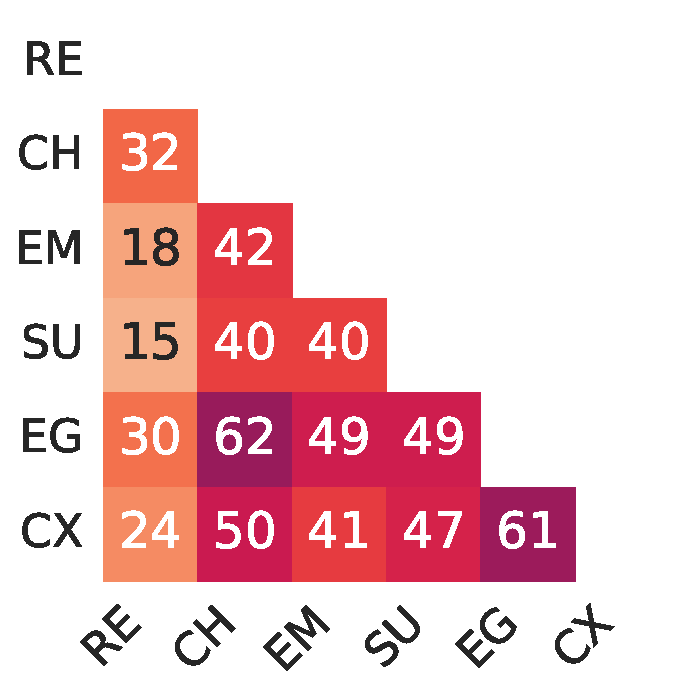
\includegraphics[width=\columnwidth]{pictures/criteria_story_kendall.pdf}
            \caption{Overall absolute Kendall correlations ($\times$100) between human criteria.}
            \label{fig:overall_human_correlations}
        }
    \end{minipage}
    \hspace{0.2cm}
    \begin{minipage}{0.45\columnwidth}
        \alt<2>{
            Moderate to weak overall correlations: our criteria evaluate \textbf{distinct aspects of storytelling} which cannot be regrouped in fewer criteria.
        }{
            \centering
            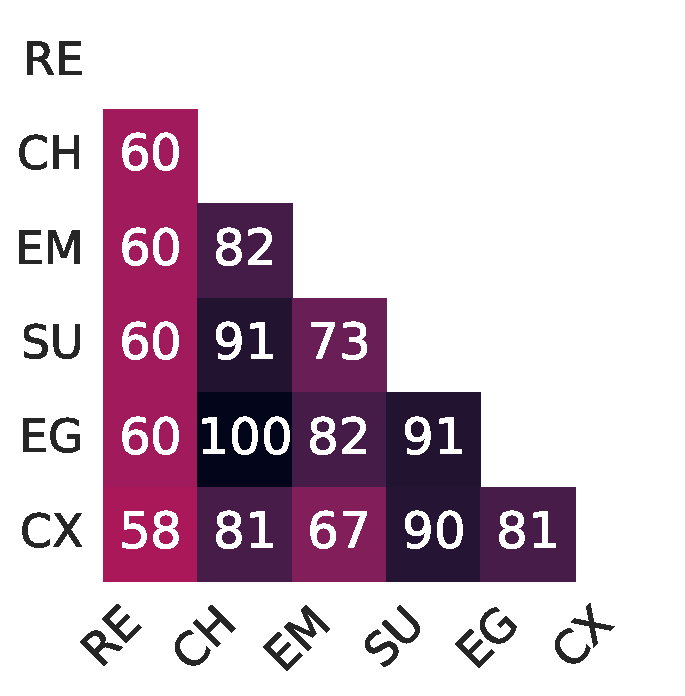
\includegraphics[width=\columnwidth]{pictures/criteria_system_kendall.pdf}
            \caption{System-level absolute Kendall correlations ($\times$100) between human criteria.}
            \label{fig:system_level_human_correlations}
        }
    \end{minipage}
    \end{figure}
\end{frame}

\begin{frame}{Performance of {\asg} Systems}
    \begin{table}[h!]
        \tiny
        \centering
        \begin{tabular}{l@{\hskip 1em}r@{\hskip 1em}r@{\hskip 1em}r@{\hskip 1em}r@{\hskip 1em}r@{\hskip 1em}r@{\hskip 1em}r}
        \toprule
        Model & \multicolumn{1}{c}{{\myre}} & \multicolumn{1}{c}{{\mych}} & \multicolumn{1}{c}{{\myem}} & \multicolumn{1}{c}{{\mysu}} & \multicolumn{1}{c}{{\myeg}} & \multicolumn{1}{c}{{\mycx}} & \multicolumn{1}{c}{Average} \\
        \midrule
        Human          &  \result{4.17}{0.14} & \result{4.43}{0.10} &  \result{3.22}{0.14} &  \result{3.15}{0.15} &  \result{3.88}{0.12} &  \result{3.73}{0.13} & \result{3.76}{0.06} \\
        \midrule
        \bertgen &  \result{2.46}{0.16} &  \result{3.14}{0.16} &  \result{2.28}{0.13} &  \result{\textbf{2.09}}{0.13} &  \result{2.67}{0.12} &  \result{2.41}{0.11} & \result{2.51}{0.06} \\
        \ctrl           &  \result{2.54}{0.16} &  \result{2.93}{0.16} &  \result{2.26}{0.13} &  \result{1.93}{0.12} &  \result{2.53}{0.12} &   \result{2.23}{0.10} & \result{2.40}{0.06} \\
        \gpt            &   \result{2.40}{0.16} &  \result{\textbf{3.22}}{0.15} &  \result{\textbf{2.37}}{0.12} &  \result{\textbf{2.13}}{0.13} &  \result{2.76}{0.13} &  \result{2.49}{0.12} & \result{2.56}{0.06} \\
        \gptt          &  \result{\textbf{\textcolor{blue}{2.81}}}{0.16} &  \result{\textbf{3.29}}{0.14} &  \result{\textbf{\textcolor{blue}{2.47}}}{0.12} & \result{\textbf{2.21}}{0.13} &  \result{\textbf{2.86}}{0.12} &   \result{2.68}{0.10} & \result{\textbf{2.72}}{0.06} \\
        \gpttag    &  \result{\textbf{2.67}}{0.16} &  \result{\textbf{\textcolor{blue}{3.31}}}{0.15} &  \result{\textbf{\textcolor{blue}{2.47}}}{0.12} &  \result{\textbf{\textcolor{blue}{2.22}}}{0.13} &  \result{\textbf{\textcolor{blue}{2.92}}}{0.12} &   \result{\textbf{\textcolor{blue}{2.80}}}{0.11} & \result{\textbf{\textcolor{blue}{2.73}}}{0.06} \\
        \roberta        &  \result{2.54}{0.16} &  \result{3.22}{0.16} &  \result{2.27}{0.12} &  \result{\textbf{2.12}}{0.13} &  \result{2.74}{0.12} &  \result{2.41}{0.11} & \result{2.55}{0.06} \\
        \xlnet          &  \result{2.39}{0.17} &  \result{2.88}{0.16} &   \result{2.10}{0.12} &  \result{1.95}{0.12} &  \result{2.46}{0.13} &  \result{2.36}{0.11} & \result{2.36}{0.06} \\
        \midrule
        \fusion         &  \result{2.09}{0.16} &  \result{2.86}{0.16} &  \result{1.99}{0.12} &  \result{1.72}{0.12} &  \result{2.27}{0.14} & \result{ 1.92}{0.11} & \result{2.14}{0.06} \\
        \hint           &  \result{2.29}{0.16} &  \result{2.38}{0.16} &  \result{1.74}{0.13} &  \result{1.56}{0.11} &  \result{1.75}{0.12} &   \result{1.45}{0.10} & \result{1.86}{0.06}\\
        \tdvae         &  \result{2.51}{0.16} &  \result{2.99}{0.15} &  \result{2.07}{0.11} &   \result{\textbf{2.10}}{0.12} &  \result{2.59}{0.12} &  \result{2.49}{0.11} & \result{2.46}{0.06} \\
        \bottomrule
        \end{tabular}
        \caption{Average system ratings per criterion with 95\% confidence interval. Higher is better.}
        \label{tab:system_averages}
    \end{table} 
    Human stories are rated much more highly than generated stories by human annotators. {\gptt} is the best system overall.
\end{frame}

\begin{frame}{Adding Large Language Models}
    We use LLMs to produce new stories for {\hanna}.\\
    We perform several annotation experiments: we ask LLMs to rate stories \wrt\ to our criteria with different Eval-Prompts (\ie, the prompt that is given as input to the {\llm}).\\
    We produce:
    \begin{itemize}
        \item \textbf{ASE}: $\sim$150k rating and explanation annotations using Llama models (Beluga-13B, Llama-13B, Mistral-7B) and ChatGPT;
        \item \textbf{ASG}: 480 stories generated by Llama models (Platypus2-70B, Llama-30B, Beluga-13B, Mistral-7B) with corresponding LLM annotations (excluding ChatGPT) to expand the \hanna\ corpus.
    \end{itemize}
\end{frame}

\begin{frame}{ASE Methodology with LLMs}
    We first provide the model with a story-prompt and a matching story. Then, we use four different Eval-Prompts:
    \begin{itemize}
        \item \textbf{Eval-Prompt 1} (simple rating): we ask the model to rate the story on a scale from 1 to 5 on one of our six criteria;
        \item \textbf{Eval-Prompt 2} (rating with explanation): Eval-Prompt 1 + we ask the model to explain its answer;
        \item \textbf{Eval-Prompt 3} (rating with explanation and guidelines): Eval-Prompt 2 + the detailed guidelines from our original human annotation protocol;
        \item \textbf{Eval-Prompt 4} (rating with explanation and human story): Eval-Prompt 2 + the human story associated with the same story-prompt. We explicitly tell the model that the human story is only given for reference purposes.
    \end{itemize}
\end{frame}

\begin{frame}{ASE Experiments}
    \begin{figure}
        \centering
        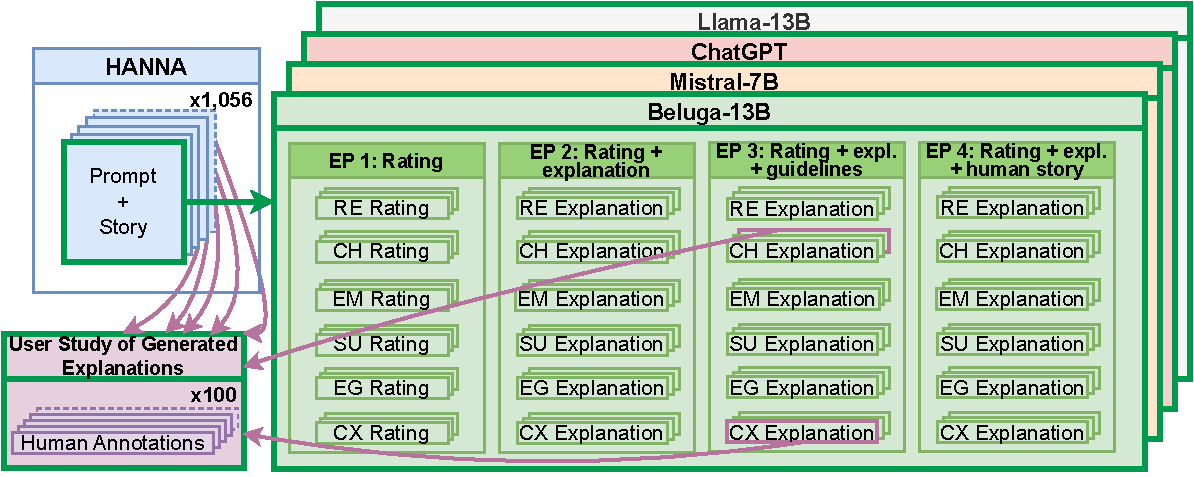
\includegraphics[width=\columnwidth]{pictures/llm_schema.pdf}
        \caption{Schema of the performed ASE experiments. ``EP'' means ``Eval-Prompt''.}
        \label{fig:llm_schema}
    \end{figure}
\end{frame}

\begin{frame}{LLM Performance at ASG}
    \begin{table}[!h]
        \tiny
        \centering
        \begin{tabular}{lccccccc}
        \toprule
        \textbf{Model} & \textbf{RE} & \textbf{CH} & \textbf{EM} & \textbf{SU} & \textbf{EG} & \textbf{CX} \\
        \midrule
        Human             &  \result{3.37}{0.12} &  \result{3.55}{0.11} &  \result{3.42}{0.11} &  \result{3.11}{0.13} &  \result{3.58}{0.10} &  \result{3.48}{0.10} \\
        \midrule
        Platypus2-70B     &  \result{4.09}{0.05} &  \result{4.31}{0.05} &  \result{3.92}{0.06} &  \result{\textbf{\textcolor{blue}{3.69}}}{0.07} &  \result{4.19}{0.05} &  \result{3.88}{0.05} \\
        Llama-30B &  \result{\textbf{\textcolor{blue}{4.19}}}{0.05} &  \result{\textbf{\textcolor{blue}{4.38}}}{0.04} &  \result{\textbf{\textcolor{blue}{4.04}}}{0.06} &  \result{\textbf{3.63}}{0.09} &  \result{\textbf{\textcolor{blue}{4.31}}}{0.05} &  \result{\textcolor{blue}{\textbf{3.98}}}{0.05} \\
        Beluga-13B        &  \result{4.06}{0.08} &  \result{4.10}{0.06} &  \result{3.75}{0.08} &  \result{3.54}{0.08} &  \result{3.90}{0.08} &  \result{3.69}{0.07} \\
        Mistral-7B    &  \result{4.12}{0.05} &  \result{4.25}{0.05} &  \result{3.86}{0.06} &  \result{3.56}{0.08} &  \result{4.11}{0.05} &  \result{3.82}{0.04} \\
        Llama-7B      &  \result{4.07}{0.06} &  \result{4.24}{0.05} &  \result{3.90}{0.06} &  \result{3.58}{0.06} &  \result{4.09}{0.05} &  \result{3.79}{0.05} \\
        GPT-2             &  \result{2.57}{0.13} &  \result{2.36}{0.11} &  \result{2.72}{0.11} &  \result{2.59}{0.14} &  \result{2.67}{0.12} &  \result{2.89}{0.12} \\
        HINT              &  \result{1.57}{0.10} &  \result{1.31}{0.07} &  \result{1.59}{0.10} &  \result{1.49}{0.10} &  \result{1.58}{0.09} &  \result{1.43}{0.08} \\
        \bottomrule
        \end{tabular}
        \caption{Average Beluga-13B ratings for Eval-Prompt 1 with 95\% confidence interval. Higher is better.}
        \label{tab:average_beluga_ratings}
    \end{table}
    Larger models (Platypus-70B, Llama-30B) are more highly rated by Beluga-13B. However, we need to confirm that LLMs are reliable proxies for human evaluation.
\end{frame}

\begin{frame}{Summary}
    \textbf{RQ2: How good are existing models at generating stories?}
    \begin{itemize}
        \item We built HANNA, a corpus containing 1,536 stories generated by 15 different systems (1 human, 3 ASG-specific, 7 pretrained LMs, 4 LLMs);
        \item All non-LLM stories were rated by 3 human annotators \wrt\ our 6 criteria;
        \item Non-LLM models are noticeably below human performance according to human raters;
        \item All stories were rated by 3 or 4 different LLMs with 4 different Eval-Prompts;
        \item LLMs seem to perform as well as human writers for this specific setting, according to Beluga-13B ratings.
    \end{itemize}
\end{frame}